\documentclass[10pt,a4paper]{article}
\usepackage[utf8]{inputenc}
\usepackage[parfill]{parskip}
\usepackage[section]{placeins}
\usepackage{graphicx}
\usepackage{array}
\usepackage{tabularx}
\usepackage[scientific-notation=true]{siunitx}
\usepackage{amsmath}

\author{Christoph Emunds (i6146758)\\Dominik Nerger (i6146759)}
\title{Autonomous Robotic Systems\\Bayes Filter}
\date{\today}

\begin{document}
	\maketitle
	
	\tableofcontents
	
	\section{Introduction}
	The Bayes filter, in the context of mobile robot localization also called \textit{Recursive Bayesian Estimation}, uses sensor measurements and a mathematical process model to estimate an unknown probability density function recursively over time.	This document describes the implementation of a Bayes filter in the Robot Operating System (ROS) framework and reflects on the filter's performance with regard to its localization capabilities in different situations. The world in which the robot is situated consists of a corridor with several doors.
	
	%This report is part of the third assignment for the course Autonomous Robotic Systems. In this report, we present our implementation of a Bayes Filter for a world model containing a corridor with several doors. Furthermore, we discuss the results that we obtained.	
		
	\section{The world model}
	The environment the robot is situated in consists of a corridor with several doors. The corridor is discretized into ten cells, which can be traversed either from left to right or vice versa. The cell the robot is located in, together with the direction it is facing, make up a belief state, which results in 20 possible states. There is no information that needs to be remembered to calculate the next belief state, so we can assume that the state is complete and that the Markov assumption holds.
	
	%Therefore, the world model needs to store information about 20 states. It is necessary that through the sensing measurements it can be deduced which states match the measured state, because this needs to be used in the calculations for the sensing update.
	
	The wall layout for each state is represented with an enumeration. This enumeration contains the four values \textit{L},\textit{LR},\textit{LRF} and \textit{R}. The characters express whether a wall has been measured to the left\textit{(L)}, to the right\textit{(R)} or in front\textit{(F)} of the robot, with a combination indicating that multiple walls have been found. Therefore, the world model is represented through a vector of size 20 and information about which measurements should be true in each state is contained in the respective enumeration value, e.g. for state $x_9$ the value is \textit{LRF}.
	
	\section{The Bayes filter}
	The Bayes filter is initialized with a uniformly distributed belief state. Sine there are 20 states, this results in an initial probability of $p(x_i)=\frac{1}{20}=0.05$ for each state. Afterwards the probabilities for the next belief state are calculated by alternating the \textit{control update} and the \textit{measurement update} step.
	
		\subsection{Control update}
		%Clarify: Is belief state the probability of a certain cell or a certain probability configuration for each cell?
		The control update is executed whenever the robot moves forward or makes a 180 degree turn. The belief state $\overline{bel}(x)$ represents the next belief state before the measurement is taken into account and is calculated according to the following formula:
		\begin{displaymath}
			\overline{bel}(x) = \sum p(x|u,x')bel(x')
		\end{displaymath}
		
		To practically calculate the new belief $\overline{bel}(x)$ after the \textit{move forward} command, we take a belief state $x_i$ and consider the states $x_i'$, $x_{i-1}'$ and $x_{i-2}'$, from which $x_i$ can be reached. The probabilities of these three possible starting locations is weighted according to the given transition probabilities and summed up. For the \textit{move forward} command, this equates to:
		%Bin mir nicht so sicher, ob das hier so richtig ist. Müssen wir nochmal diskutieren
		\begin{displaymath}
			\overline{bel}(x_i) = 0.8\times p(x_{i-1}') + 0.1\times p(x_{i-2}') + 0.1\times p(x_i')
		\end{displaymath}
		
		However, two extra cases have to be considered. The first extra case are the states $x_i$ for which ($i \mod{10} = 0$) holds true, i.e. the states $x_0$ and $x_{10}$. Since the world is not cyclic, there are no states $x_{i-1}'$ and $x_{i-2}'$ from which the states $x_0$ and $x_{10}$ could be reached. Therefore, the probability of these two states is calculated according to
		\begin{displaymath}
			\overline{bel}(x_i) = 0.1\times p(x_i')
		\end{displaymath}
		
		The second extra case are the states $x_i$ for which ($i \mod{10}=1$) holds true. Explicitly, these are the states $x_1$ and $x_{11}$. Similarly to the above reasoning, there are no states $x_{i-2}'$ from which the states $x_1$ and $x_{11}$ could be reached. Therefore, the probability of these two states is calculated according to		
		\begin{displaymath}
			\overline{bel}(x_i) = 0.8\times p(x_{i-1}') + 0.1\times p(x_i')
		\end{displaymath}
		
		%Diesbezüglich sollten wir vielleicht nochmal die anderen fragen
		Due to these extra cases, the resulting values for $\overline{bel}(x)$ do not sum to a probability of 1 anymore and need to be normalized again.
		
		The new belief state for the \textit{turn} command is calculated according to		
		\begin{displaymath}
			\overline{bel}(x_i) = 0.9\times p(x_{N-1-i}') + 0.1\times p(x_i')
		\end{displaymath}
		where $N$ is the number of belief states.
		
		\subsection{Measurement update}
		The belief state after incorporating the measurement probability is represented by
		\begin{displaymath}
			bel(x)=\eta p(z|x)\overline{bel}(x)
		\end{displaymath}
		where $\overline{bel}(x)$ is the previously calculated belief state after the control update but before taking the measurement into account, $p(z|x)$ is the probability that the measurement $z$ has been taken in the state $x$ and $\eta$ is a normalization constant.
		
		To calculate the new belief state $bel(x)$, a measurement is taken. This measurement consists of checking whether there is a wall to the left, to the right and in front of the robot. Then, for each belief state $x_i$ it is checked whether the measurement agrees with the layout of the current cell, i.e. if the value for the boolean variables \verb|wall_left|, \verb|wall_right| and \verb|wall_front| corresponds to state $x_i$ having a wall to the left, right or front, respectively. If the measurement agrees with there being a wall, the probability for being in the corresponding state is multiplied by a factor of $0.6$. The probability for every other state is multiplied by $0.2$.
		
		During this first loop, the resulting products are also summed up. In a second loop, the calculated values are then divided by the sum, such that they represent proper probabilities again, normalizing the belief states.
	
	\section{Results}	
	Most states in the corridor have a wall on both sides, which makes them indistinguishable. When issuing the \textit{measurement} command in a state that has a door on either the left or the right side, the probabilities of the states containing a door on the specific side rise. Multiple continuous measurements cause the robots confidence for being in one of these states to grow.
	
	Furthermore, the same holds true when a wall is measured in front of the robot. Then the probability that the robot is in one of the two states that should measure a wall in front rise severely.
	
	%States that are opposite to a door are also easily identified.
	Noise in sensing, moving and turning cause the certainty to drop significantly. If the robot does not move forward or takes two steps at once, the state with the highest probability is likely to be false. The same holds for wrong measurements while sensing the walls. The robot is able to recover from that when reaching another location that is easily distinguishable from the rest and correct measurements. If a sequence of wrong measurements and/or wrong steps occur, it is possible that the robot assigns the highest probability to a wrong state. 
	
	Most of the time the robot tracks two hypotheses. After taking measurements at two unique locations in a row, most of the probability focusses on only one state. This certainty is kept when alternating movement (including \textit{move forward} and \textit{turn}) and sensing, until one of these actions fails.
	
	Consider the example case in which the robot should move one cell forward. If it fails to do so and stays at its location, still $80\%$ of the probability of the current state are convolved to the next state. However, after reaching the next state that either has a door, is opposite to a door or has a wall in front of the robot, the probability quickly focusses on the right state again if the sensing measurements are correct, allowing for a quick recovery.
	
	The measurements in Figure~\ref{fig:4stepsNoNoise} show the robot, which has taken four steps forward with a sensing update after each step and no noise. As can be seen, the robot is certain that it is in state \textit{$x_9$}, which is correct. The probability for that is around \textit{0.38}. This result can be recreated because it is deterministic.
	
	\begin{figure}[h]
		\centering
		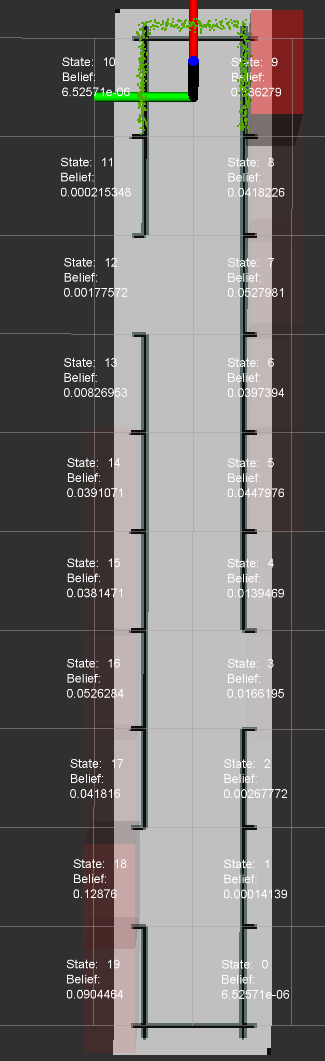
\includegraphics[scale=0.9]{data/4stepsforward.png}
		\caption{Four movement/sensing updates without noise}
		\label{fig:4stepsNoNoise}
	\end{figure}
	
	For the measurements in Figure~\ref{fig:4stepsNoise}, the robot took four steps forward with a sensing update after each step as well. However, this time both the movement and measurement noise were activated. Due to the noise, the robot is uncertain about its state, because the probabilities for states \textit{$x_5$}, \textit{$x_9$} and \textit{$x_{14}$} do not differ that much. State \textit{$x_9$}, which is the correct state, still has the highest probability, but the robot is not as certain as in the example shown in Figure~\ref{fig:4stepsNoise}.
	
	\begin{figure}[h]
		\centering
		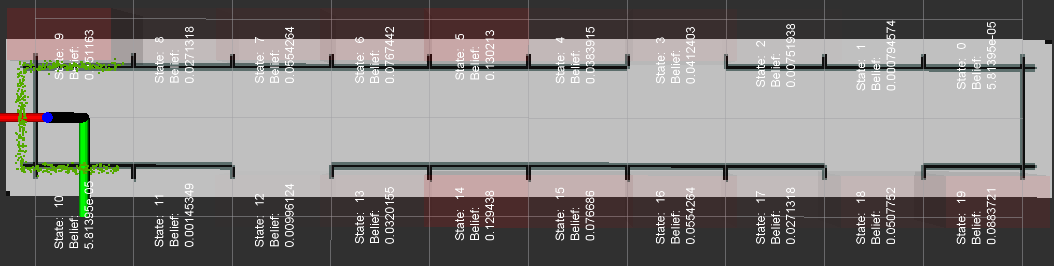
\includegraphics[scale=0.9]{data/4stepsforwardNoise.png}
		\caption{Four movement/sensing updates with noise}
		\label{fig:4stepsNoise}
	\end{figure}
	
	\section{Conclusion}
	The results show that our implementation behaves according to the theory of Bayes filters. If the robot reaches a location that it can distinguish from most of the other locations, its certainty for being in one of these states grows. After reaching a second location that differs from most of the other locations, most of the probability focusses on the right state. The implementation is also fairly robust to noise in the measurements and actions of the robot, but if a sequence of wrong measurements occur the robot might favor a wrong state for a period of time, after which it will be able to recover if distinguishable locations with no wrong measurements occur.
	
\end{document}